\section{Security isolation}
\label{sec:linux:security}

\issuedone{1.1.d}{describe the security isolation story for Linux hosts}
\graphene{} separates OS features from security isolation.
This section explains the Linux host design for isolating mutually untrusting applications, with a reduced attack surface for protecting Linux kernels.
The discussion starts with the security guarantees and threat model, followed by the technical details of security isolation on a Linux host.



\subsection{Goals and threat model}

The security isolation model of \graphene{} ensures that mutually-untrusting applications cannot interfere with each other.
A goal of \graphene{} is to provide security isolation with comparable strength as
running applications in separate VMs.
When running two unrelated applications on the same machine,
the security requirement
of the OS involves not only blocking unauthorized access under normal circumstance,
but also preventing an application
from maliciously exploiting OS vulnerabilities to attack the other application.
Because a modern OS, such as Linux or Windows, contains a rich of features and APIs,
it is difficult to eliminate OS vulnerabilities
or even just to verify whether an OS contains any vulnerabilities. 
A Linux container~\cite{lxc}
does provide a separate OS view for each application,
but still relies on the correctness of the whole Linux kernel to enforce security isolation.
On the other hand, a VM or a \libos{}
isolates the whole OS kernel or a part of the kernel in an unprivileged guest space
for each application.
The security isolation model prevents
any vulnerabilities inside the VM or the \libos{} from compromising the host kernel and other applications.



\graphene{} enforces security isolation %between applications
by separating 
backward-compatible OS features from security mechanisms.
A Linux kernel exports a wide range of \linuxapis{},
either as a legacy of previous kernels or as new programmability features. % of newer kernels.
By implementing OS features in a \libos{},
\graphene{} reduces the attack surface of a Linux kernel
to a small amount of \linuxapi{} corner cases.
%to implement \thehostabi{}.
%If a machine only runs applications in \graphene{},
%a Linux developer can try to carve out a minimal Linux kernel, containing only features needed by the Linux PAL.
A reduced attack surface
eliminates majority of execution paths inside a Linux kernel in which a malicious application can explore for vulnerabilities.
The complexity of Linux features and APIs exported by a \libos{} is unrelated with the attack surface of the host kernel,
unless the \libos{} asks for additional \hostapis{}.
A Linux developer can even carve out a minimal Linux kernel with only the features needed by the Linux PAL,
similar to shrinking a Linux kernel to a microkernel.
Otherwise, \graphene{} depends on the host security mechanisms to restrict a \libos{} from accessing unauthorized \linuxapis{} and resources upon an unmodified Linux kernel.





The Linux PAL installs a {\bf \linuxapi{} filter} and a {\bf reference monitor}
for restricting the \linuxapis{}, files, RPC streams, and network addresses
accessed by a \picoproc{}.
The Linux PAL requires \hostsyscallnum{} \linuxapis{} in total
for implementing both required and optional \hostapis{}.
A \linuxapi{} filter, such as the Linux \seccomp{} filter~\cite{seccomp},
can restrict the \linuxapi{} access of an application
to only a small subset of all the \linuxapis{}, with additional constraints on the parameters and optional flags permitted for each \linuxapi{}.
%The \linuxapi{} filter
%forbids an application from invoking any \linuxapis{}
%that will interfere other \picoproc{} or increase the risk of exploitation in the host kernel.
A reference monitor further examines the arguments of permitted \linuxapis{} to restrict the host resources accessed by an application, based on security policies configured in a manifest file~\cite{hunt07rethink}.
The \linuxapi{} filter and the reference monitor
significantly limit the ability of an untrusted \graphene{} \picoproc{} to interfere with the rest of the system,
preventing the risk of exposing any unknown vulnerabilities
on a kernel path never exercised by the \linuxapi{} footprint of \graphene{}.



\graphene{} contributes a multi-process security model 
based on a {\bf sandbox},
or a set of mutually-trusting \picoprocs{} running inside an isolated container.
The reference monitor permits picoprocesses within the same sandbox
to communicate over RPC streams,
allowing the \libos{} to share and coordinate any states
to create an unified OS view.
If two \picoprocs{} belong to different sandboxes,
the reference monitor will block any attempt of connecting RPC streams
between the \picoprocs{}
The access control over RPC streams
enforces an all-or-nothing security isolation model:
either two \picoprocs{} are in the same sandbox and share all the \libos{} states; or they are separated in two sandboxes and share nothing.
Even though the \libos{} instance can span its state across multiple \picoprocs{},
a host kernel needs not to examine the accesses to shared \libos{} states, but still enforces security isolation between sandboxes.




Files and network addresses
are the only host resources allowed to be shared across sandboxes,
using well-studied, explicit rules.
For sharing files, the reference monitor restricts the file access of a \picoproc{}
within a few host file or directories,
creating a restricted view of the local file system
(close to Plan 9's unionized file system views~\cite{pike90plan9}).
The file rules
in a manifest are similar to the policies of a {\bf AppArmor profile}~\cite{apparmor};
for each permitted file or directory,
a developer specifies the URI prefix and the permitted access type, either as read-only or readable-writable. %, within the target file or directory.
For sharing network addresses,
the reference monitor restricts a \picoproc{} from connecting through a local address or connecting to a remote address,
using {\bf iptables-like firewall rules}~\cite{iptablesman}.
Each network rule in a manifest
specifies the local or remote IP address and port range that a \picoproc{} is permitted to bind or connect a network socket.
The rules in a manifest file
specify a minimal list of files and network addresses that a \picoproc{} needs to access, and are largely based on existing security policies (e.g., AppArmor profiles, firewall rules).





\paragraph{Threat model (details).}
When running on a normal Linux host (without SGX or other security hardware), \graphene{} assumes a trusted host kernel and reference monitor.
All the components inside the kernel space, including the \code{gipc} kernel module for bulk IPC, and the reference monitor,
are fully trusted by the other parts of the host kernel and the \graphene{} \picoprocs{}.
%which mediates all system calls with effects outside of a picoprocess's address space,
%such as file {\tt open} or network socket {\tt bind} or {\tt connect}.
On the other hand,
the host Linux kernel does not trust the \picoproc{}, including the Linux PAL, a \thelibos{} instance, \glibc{}, and the application.
The \linuxapi{} filter and reference monitor
initialized before an application starts running
defend the whole host kernel from malicious \linuxapis{} invoked by a \picoproc{}.



All the components running within a \picoproc{}, including the Linux PAL, the \libos{} (\thelibos{}), \glibc{} libraries, and the application,
mutually trust each other. %, because all these components
%execute in the same guest address space.
Without internal sandboxing, the Linux PAL or \thelibos{}
cannot protect its internal states or control flows from an application.
Although some scenarios might require protecting the PAL or \thelibos{}
from the application,
\graphene{} only restricts the adversary
within a \picoproc{};
in other word, an adversary
only compromises the \libos{} in the same \picoproc{},
but can never interfere the host kernel 
or other unrelated \picoprocs{}.



For a multi-process application,
\graphene{} assumes that the \picoprocs{} 
%launched by the same application instance
running inside the same sandbox
trust each other and that all untrusted code run in sandboxed \picoprocs{}.
\graphene{} assumes the adversary can run arbitrary code inside
one or multiple \picoprocs within a sandbox.
The adversary can exploit any vulnerabilities in the \libos{}
or IPC protocol,
to propagate the attack to other \picoprocs{}.
\graphene{} ensures that
the adversary cannot interfere with any victim \picoprocs{}
in a separate sandbox.
A sandbox strictly isolates the coordination of \thelibos{} instances;
%if the only shared kernel abstractions are byte streams and files, 
the reference monitor ensures
that there is no writable intersection between sandboxes, so that
the adversary cannot interfere with any victim \picoprocs{}.


%%% The only processes allowed to run as standard kernel processes (non-\graphene{}) 
%%% are the reference monitor and
%%% system administration utilities that need more kernel interfaces than the \pal{} ABI provides.
%%% Ensuring that a collaborating picoprocess correctly implements
%%% some function (such as receiving a signal),
%%% as well as preventing exploitation of vulnerabilities in picoprocesses
%%% are beyond the scope of this work.

\graphene{} reduces the attack surface of the host Linux kernel, but does not change the trusted computing base; however, reducing the effective \linuxapi{} table size of a \picoproc{} does facilitate adoption of a smaller host kernel.
This thesis leaves the creation of a smaller host kernel for future work.

\subsection{System call restriction}
\label{sec:linux:security:syscall-restriction}


\graphene{} reduces the host ABI to \palcallnum{} calls
and the Linux \linuxapi{} footprint to \hostsyscallnum{} \linuxapis{}.
To reduce the effective attack surface to a Linux host,
the Linux host restricts a \picoproc{} from accessing any \linuxapis{} that are not part of the ordinary footprint of a Linux PAL.
The \linuxapi{} restriction on Linux focuses on blocking most of the \linuxapis{}
that interferes with other processes.
The remaining permitted \linuxapis{} with external effects are checked by 
the reference monitor (see Section~\ref{sec:linux:security:ref-monitor}).
 
%% dp: Meh
%%% Any picoprocess implementation 
%%% must restrict access to the host system call table,
%%% generally by blocking system calls in the host kernel~\cite{porter11drawbridge}
%%% or using {\tt ptrace}~\cite{xax}.


%The \pal{} is a host-provided library which implements \palcalls{} generic kernel ABIs,
%implemented using 
%These native system calls include {\tt ioctl} with 5 opcodes exclusively used by \graphene{} kernel extensions.

%This section describes how we adapt recent Linux sandboxing techniques 
%to \graphene{}.


%all allowed system calls with potentially external effects.

%%% For instance, an attempt to open a file will be checked by the reference monitor
%%% to see if the file is included in the sandbox definition, specified in the manifest
%%% with required permissions.
%%% Once the file handle is open, the \pal{} is then allowed to issue an {\tt mmap} or {\tt read}
%%% on the handle, as this operation can only affect the picoprocess address space
%%% or  file, which was already checked.

%Because the \pal{} is in the same address space as the application code, it is not
%trusted to enforce any security policies, and our threat model assumes that
%the \pal{} can be compromised by the adversary.
%Thus, the host kernel 
%only permits system calls that appear in the \pal{}'s source code and, through the reference monitor, further inspects calls that can have external effects.

%\begin{figure}[t!]
%\centering
%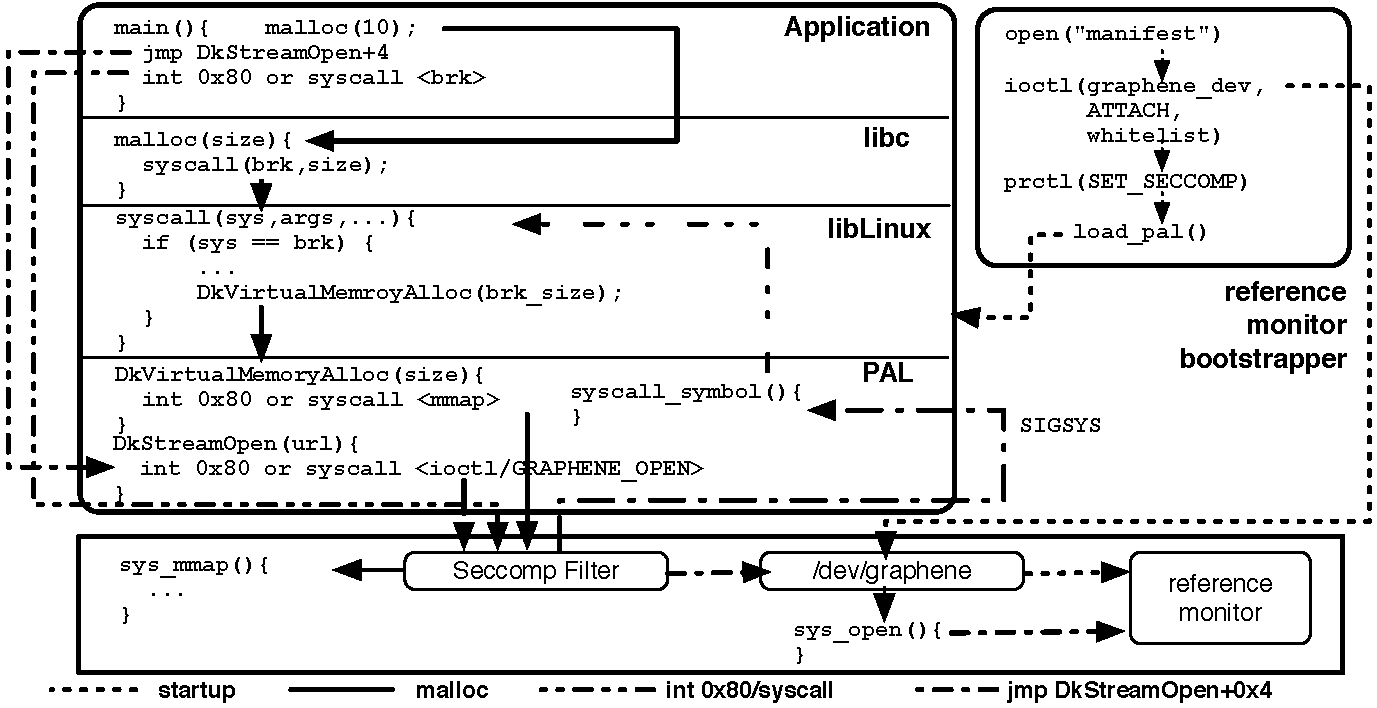
\includegraphics[width=\linewidth]{syscall-restriction.pdf}
%\footnotesize
%\caption[System call restriction approach in sysname{}]
%{System call restriction approach. The reference monitor loads policies into the LSM at startup.  A \graphene{} application requests OS services in three different ways. 
%In the normal case (first line of {\tt main}), {\tt malloc} is invoked causing the invocation of {\tt brk} ({\tt libLinux}) and {\tt mmap} in the \pal{}. In the second line, the application jumps to an address in \pal{}, which is permissible.
%Files are accessed through {\tt ioctl} to {\tt /dev/graphene} and checked by reference monitor.
%The third line invokes {\tt brk} with an {\tt int} instruction, which is redirected to the {\tt libLinux} function.}
%\label{fig:graphene:syscall-restriction}
%\end{figure}



\issuedone{1.3.d}{extend the discussion of \seccomp{} filter}
\graphene{} restricts the host \linuxapis{} 
using a \seccomp{} %(SECure COMPuting)
filter~\cite{seccomp}, a feature introduced in Linux 2.6.12.
% a recent Linux system call filtering mechanism, called 
A \seccomp{} filter allows a Linux process to install an immutable Berkeley Packet Filter (BPF) program
that specifies allowed \linuxapis{}, as well as specifies
the consequence of invoking certain \linuxapis{}, such as creating a \code{ptrace} event or raising a \code{SIGSYS} signal.
The BPF grammar is rich enough to filter scalar argument values,
such as only permitting specific opcodes for \syscall{ioctl},
as well as filter certain register values, such as blocking \linuxapis{} from program counters (i.e., \code{RIP} register values) outside of the Linux PAL.
%This feature is particularly salient in the case of {\tt ioctl},
%where the \pal{} uses 5 out of over 400 opcodes for our bulk IPC module and sandbox creation;
%our BPF rules will block any other {\tt ioctl} opcode.
The current \seccomp{} filter installed by the Linux PAL contains \seccomplines{} lines of straightforward BPF macros.  %Experiments show that adding more precise argument checks has no significant impact on \linuxapi{} latency.
Once a \seccomp{} filter is installed in a process,
the filter intermediates
every \linuxapis{} from the process and its future children, and guarantees the processes can never bypass the restriction.
The Linux PAL uses \code{SIGSYS} signals to capture rejected \linuxapis{},
and can either terminate the whole application or
redirect the \linuxapi{} to \thelibos{}.
The consecutive steps of \linuxapi{} redirection are described in Section~\ref{sec:libos:syscall-redirection}.



Developing a \seccomp{} filter presents several technical challenges.
First, a filter must restrict consecutive \picoprocs{}
to install a new filter the reverts the \linuxapi{} restriction.
%A \seccomp{} filter is installed using the \syscall{prctl} \linuxapi{}, so
Blocking the \syscall{prctl} \linuxapi{} in a \seccomp{} filter will prevent further installation of \seccomp{} filters.
Second, the BPF grammar can only filter certain values or ranges of a register.
The filter needs to
ensure that only the Linux PAL can invoke \linuxapis{};
however,
for satisfying the dynamic loading behavior of \thehostabi{},
the Linux PAL
is built as a shared library loaded at an address randomized by the Linux ASLR (Address Space Layout Randomization) feature.
If a filter only permits a specific range of program counters,
a child \picoproc{}
will load the Linux PAL at another randomized address,
and the inherited filter will restrict the child \picoproc{} to invoke any \linuxapis{}.
The Linux PAL introduces a small, initial loader
loaded at a fixed address
within each \picoproc{} and permitted to invoke \linuxapis{}.
Finally, a \seccomp{} filter
cannot check a string argument, such as a file path for \syscall{open} or a network address for \syscall{bind}.
Checking a string argument requires
involves reading user memory of unknown sizes and string comparison, and the BPF grammar only allows checking an argument arithmetically.
Filtering permitted file paths and network addresses
must rely on a trusted reference monitor (see Section~\ref{sec:linux:security:ref-monitor}).
%In order to avoid the overhead of trapping to the reference monitor on 
%every use of {\tt open}, {\tt stat}, {\tt bind} or {\tt connect} system calls, we instead 
%force picoprocess to only use {\tt ioctl} system call to \graphene{} special device ({\tt /dev/graphene}) as alternative interface these system calls. Direct access to these system calls are banned by seccomp filter.
%extend AppArmor~\cite{apparmor} 
%to enforce file system isolation in the kernel.



The \seccomp{} filter blocks  unauthorized \linuxapis{}
from anywhere inside a \picoproc{}.
Even if none of the application binaries contains any \assembly{syscall} or \assembly{int \$80} instruction,
a piece of malicious application code can always bypass the Linux PAL
to invoke unauthorized \linuxapis{}.
The application code can simply
jump to a \assembly{syscall} instruction inside the Linux PAL,
or corrupt a returned address on the current stack to launch a ROP (return-oriented programming) attack.
Even if the Linux PAL is hidden or isolated from the application,
an adversary can always leverage a gadget, a byte sequence that resembles the target instruction, within an executable or a library.
Therefore, the \seccomp{} enforces both program-counter-based 
and argument-based restrictions
to block unauthorized \linuxapis{} from both the Linux PAL and the rest of \picoproc{}.


%In order to reduce the impact of bugs in the reference monitor,
%the reference monitor itself runs with a \seccomp{} filter, blocking unexpected system calls.


\paragraph{Security implications.}
Using an existing \linuxapi{} restriction mechanism like \seccomp{},
\graphene{} limits the ability of an untrusted application to attack a Linux kernel.
Ideally, since \thelibos{} only requires \thehostabi{},
\graphene{} can adopt a modified Linux kernel
that only exports \palcallnum{} \hostapis{} to each \picoproc{}.
%However, as a usability feature, \graphene{} runs \graphene{} on an unmodified Linux kernel using a Linux PAL to translate among host interfaces.
The \seccomp{} filter instead isolates a \picoproc{} on an unmodified Linux kernel,
with a reduced attack surface 
comparable to only exporting \thehostabi{}.
%The filter only permits \hostsyscallnum{} \linuxapis{} with specific flags and opcodes
%required by the Linux PAL.
According to the principle of least privilege,
each component or layer in a system should only be granted access to a minimal amount of resources or abstractions
required for performing the expected tasks.
The \seccomp{} filter only permits
a minimal amount of \linuxapis{} with specific flags and opcodes
required by the Linux PAL,
so an untrusted application
can only trigger
a limited amount of execution paths inside the host Linux kernel.
\graphene{} limits
the ability of an untrusted application to explore
known and unknown vulnerabilities
on any kernel execution paths for servicing one of the blocked \linuxapis{}.



Although a regular Linux process can also leverage a \seccomp{} filter,
\graphene{} makes a major contribution
to reduce the \linuxapi{} footprint of any large-scale application
to a fixed, small \linuxapi{} profile.
Analysis %of applications and libraries
%in the official Ubuntu repositories
shows that the \linuxapi{}  footprint of a large-scale application such as Apache or MySQL can contain more than 100 \linuxapis{}.
Since \thelibos{} has absorbed the Linux \linuxapi{} table,
running Apache, MySQL, or any other application in \graphene{} leads to at most \hostsyscallnum{} host \linuxapis{}.
As a system
running a wide range of applications
can exposes a different partial view of the \linuxapi{} table to each application,
\graphene{}
has a static \linuxapi{} profile for all applications,
allowing OS developers to focus
on testing or analyzing a small portion of execution paths and corner cases
of a Linux kernel.
\citet{sun15unpredictability}
proposes sandboxing an uncertain, potentially-malicious application
in \graphene{}
with an unpredictable \thelibos{} implementation.







\paragraph{Static binaries.}
Besides security purposes,
a \seccomp{} filter provides a compatibility feature
for redirecting hard-coded \linuxapis{}
in a statically-linked application binary.
\graphene{} leverages the \seccomp{} filter to redirect these leaked \linuxapis{}
back to \thelibos{}. 
The filter contains BPF rules to check if the program counters
invoking the \linuxapis{}
are parts of the Linux PAL.
The filter blocks \linuxapi{} invoked outside of the Linux PAL
and delivers a \code{SIGSYS} signal
to the PAL signal handler for redirecting the \linuxapis{} to \thelibos{}.



\subsection{Reference monitor}
\label{sec:linux:security:ref-monitor}

The reference monitor on a Linux host
checks the arguments of host \linuxapis{} for referencing any sharable host resources.
A host \linuxapi{} like \syscall{open}, \syscall{connect}, or \syscall{bind}
specifies a file system path or a network address
for opening a file or network stream and cannot be filtered by a \seccomp{} filter.
The host kernel trusts the reference monitor
to only permit
a list of sharable resources in a \picoproc{},
based on
rules in a manifest file.
Once the reference monitor has permitted the creation of a file or network stream,
consecutive operations on the stream
such as reading or writing data can be trusted
as long as being mediated by one of the permitted \linuxapis{}.


\begin{figure}
\centering
\begin{lstlisting}
loader.exec = file:/usr/sbin/apache2        # allow loading executable 
loader.preload_libs = file:/graphene/libLinux.so    # loading libLinux
fs.allow_ro.libc = file:/graphene/libc/     # loading modified libc
fs.allow_ro.mods = file:/usr/lib/apache2/modules/   # loading modules
fs.allow_ro.cond = file:/etc/apache2/       # reading configuration
fs.allow_rw.logs = file:/var/log/apache2/   # writing to logs
fs.allow_ro.http_docs = file:/var/www/      # reading website files
net.allow_bind.httpd = 0.0.0.0:80           # binding to local port 80
net.allow_conn.any = 0.0.0.0:1-65535        # allow any connection
\end{lstlisting}
\caption{A example of a manifest file, containing security rules for the reference monitor to permit accessing sharable resources. The manifest file is for running a Apache http server (without php and other language engines).}
\label{fig:linux:manifest-example}
\end{figure}


The reference monitor enforces simple, white-listing rules
based on security mechanisms
already familiarized by users and developers.
Figure~\ref{fig:linux:manifest-example} shows an example of resource access rules
in a manifest.
First, a manifest lists
the URI prefixes of permitted files or directories
of an application,
similar to an AppArmor profile.
The executable (\code{loader.exec}) and the preloaded \libos{} binaries (\code{loader.preload\_libs})
are permitted for read-only access by default.
The reference monitor
simply compares file URIs against each permitted URI prefix
and checks the access types;
unlike many existing security mechanisms in Linux and similar OSes, such as permission bits, Access Control Lists (ACLs), and SELinux labels,
the reference monitor does not retrieve
security policies from file metadata, but obtains the manifest from an out-of-band channel.


Manifest-based security
simplifies the inspection, authentication, and population
of security policies.
An Android application is deployed with a similar manifest,
listing the accessed files and other resources,
which users approve when installing the application.
Developers can authenticate a security policy by signing the content of a manifest.
Moreover, to run an application, a user can choose among multiple manifest files
with different levels of security privileges.



Network rules in a manifest are similar to {\bf iptables firewall rules} for defending a server or a desktop machine.
A network rule specifies a local or remote address
that the application is permitted to bind or connect a network stream.
A local or remote address
can be an IPv4 or IPv6 address (possible to specify an ``any'' address, i.e., \code{0.0.0.0} or \code{[::1]}), combined with a specific port number or range.
When an application creates a network stream,
the reference monitor checks whether the local and remote addresses
match one of the network rules.







%is implemented using {\tt ioctl} system call to a special device {\tt /dev/graphene}.
%A picoprocess is restricted by seccomp filter~\cite{seccomp} to use any {\tt open} or socket {\tt connect} and {\tt bind} system calls.
%It must use the \graphene{} special device to open or create streams,
%so the file paths or network addresses can be checked against the sandbox rules.
%The kernel module as the driver of the \graphene{} special device can coexist with any LSM such as \emph{AppArmor} or \emph{SELinux}.

The reference monitor on a Linux host
is implemented as a Linux Security Module (LSM) extended from the existing AppArmor module.
AppArmor is the default LSM of most Linux distributions,
and a Linux kernel disallows multiple LSMs (e.g., AppArmor, SELinux) to be effective simultaneously.
\graphene{} instruments
a few security hooks of the AppArmor, to add checks for file system paths
and network addresses.
The security checks of the reference monitor are stackable with other host security mechanisms.
For example, if a manifest lists a root-privileged file and the \graphene{} application runs in a unprivileged process,
existing security checks in a Linux kernel
still blocks the file access even though the reference monitor permits the access.
The drawback of the implementation
is that \graphene{} must run on a modified Linux kernel.
Linux kernels do not support loading LSM as a dynamic kernel module.
\graphene{} only replaces
the AppArmor LSM in a Linux kernel; the rest of the Linux kernel remains unchanged.


A trusted security loader initializes the reference monitor
when launching an application in \graphene{}.
When a user launches an application in \graphene{} from the command line,
the first \picoproc{} begins in a new sandbox.
The security loader
reads the manifest file given by the user,
and submits the sandbox rules to the reference monitor.
The reference monitor exports a miscellaneous device called \code{/dev/graphene}
for the security loader to submit sandbox rules using the \syscall{ioctl} \linuxapi{}.
Once the reference monitor
starts a \picoproc{} in a sandbox, neither the first \picoproc{} nor any consecutive \picoprocs{} spawned in the sandbox can ever escape the sandbox or drop the restrictions on certain resources.


\paragraph{Alternative approaches.}
Other approaches can implement the reference monitor without modifying a Linux kernel, with a trade-off of performance or development simplicity.
An approach is to implement the reference monitor as a trusted process receiving \code{ptrace} events from \graphene{} \picoprocs{}.
Using the \syscall{ptrace} \linuxapi{}, this reference monitor can retrieve user memory from the monitored \picoprocs{},
and block the \linuxapis{} which request for unpermitted resources.
Unfortunately, intercepting every \linuxapis{} with \code{ptrace} events introduces significant overhead to \hostapis{};
thus, this approach is not ideal for isolating \graphene{} applications on a Linux host.


Another approach is to translate the resource rules in a manifest file
to AppArmor or iptables rules.
As explained in previous paragraph, the file and network rules in a manifest file are similar to the file lists in an AppArmor profile and the firewall rules enforced by iptables.
Instead of implementing a \graphene{}-specific reference monitor,
\graphene{} can convert a manifest file, either statically or dynamically,
to security rules recognized by AppArmor and iptables.
This approach requires no modification
in a Linux kernel, and can benefit from
existing optimizations of AppArmor and iptable. %these security mechanisms.
\graphene{} leaves the integration with AppArmor and iptables for future work.




\paragraph{Dynamic process-specific isolation.}
A child \picoproc{} may either inherit its parent's sandbox, 
or start in a new sandbox,
by either specifying a flag to \palcall{ProcessCreate} or calling the sandboxing \hostapi{}, \palcall{SandboxSetPolicy}.
A new sandbox may obtain a subset of the original file system view,
but can never request access to new regions of the 
host file system. 
%The restrictive policy enforced on the child will be written in a new manifest file generated by the parent, and the policy will be checked by the reference monitor.
If a child \picoproc{} voluntarily moves itself to a new sandbox
using \palcall{SandboxSetPolicy},
the Linux PAL issue another \syscall{ioctl} call to \code{/dev/graphene}
to dynamically detach
the \picoproc{}
from the parent's sandbox and update sandbox rules. The reference monitor
closes existing RPC streams and prevents RPC stream creation 
across sandboxes.
%among picoprocesses
%that are not in the same sandbox.
%and restricts external connections to remote URIs according to firewall rules in the manifest.
When a process detaches from a sandbox,
the reference monitor effectively splits the original sandbox
by closing any RPC streams that could bridge the two sandboxes.


\begin{comment}
We hasten to note that program counter filtering
is only provided for backwards compatibility, not security.
An attacker can compromise the \pal{}, so system policies are enforced
externally by the reference monitor.


Dynamically redirecting system calls to {\tt libLinux} is 
less efficient than dynamically linking against
the \graphene{} libc or statically compiling {\tt libLinux} into the application.
The overhead of dynamic redirection comes from 
transferring control to the kernel, then back to 
the \pal{}, and then to {\tt libLinux}.
We leave exploration of more efficient alternatives for future work,
such as redirecting the hardware system call table to {\tt libLinux}
on a host system like Dune~\cite{belay12dune},
or dynamically rewriting parts of the static binary~\cite{hunt99detours}.
\end{comment}

%\paragraph{Example.}
%Figure~\ref{fig:graphene:syscall-restriction} illustrates three possible situations. 
%%% An unmodified Linux application is dynamically linked against the 
%%% \graphene{} {\tt libc}, 
%%% which then dynamically links its system calls from {\tt libLinux},
%%% which in turn links in the host kernel ABI from the \pal{}.
%%% The application requests OS functionality in three ways.
%An unmodified application first invokes the {\tt libc} function {\tt malloc}, which issues 
%a {\tt brk} system call to {\tt libLinux}, which requests memory 
%from the host via a {\tt Dk\-Virtual\-Memory\-Alloc} \pal{} call,
%which ultimately issues an {\tt mmap} host system call.
%The {\tt mmap} host system call is allowed by seccomp because it only 
%affects the picoprocess's address space.
%The second line of the application jumps to the \pal{} instruction that issues
%an {\tt open} system call.
%From a security perspective, this is permissible,
%as it is isomorphic to \pal{} functionality.
%In practice, this could cause
%corruption of {\tt libLinux} or application data structures,
%but the only harm is to the application itself. 
%Because this system call involves the file system, the reference monitor LSM first checks if the file to be opened is included in the sandbox definition (manifest) before allowing  the {\tt open} system call in the kernel.  
%Finally, the application uses inline assembly to issue a {\tt brk} system call;
%%in an attempt to obtain I/O port privilege; 
%because this system call was not issued by the \pal{},
%seccomp will redirect this call back to the \pal{},
%which then calls the {\tt libLinux} implementation.


Sandbox creation in \graphene{} can provide
more options than virtualization, to reflect the security policy of applications at any timing,
in the granularity of picoprocess. 
A picoprocess can voluntarily detach itself from the current sandbox, dropping its privileges,
after finishing security-sensitive operations.
If a picoprocess decides one of its children is not trustworthy, it may also start the child under a restricted manifest,
or promptly shut down RPC streams to stop sharing OS states.
The picoprocess that moves to a separate sandbox will have a restrictive view of the filesystem, and no coordination with the previous sandboxes.
Section~\ref{sec:eval:graphene} describes an experiment that improves security isolation of Apache http server without sacrificing functionality.



%We add a \pal{} call which
%permits a picoprocess to request that it be moved into a new sandbox.
%This call, as well as file system path checks, are implemented
%as extensions to the  AppArmor LSM~\cite{apparmor}.
%%We modify \sandboxmodlines{} lines in the
%%to implement this call,
%The new sandbox call closes any open stream handles that cross sandbox boundaries;
%mediate path lookups;
%and create a new broadcast stream for multi-process
% coordination (\S\ref{sec:graphene:namespaces:blocks}).
%%The reference monitor also interposes on this call so that it can 
%%mediate future stream creation.

%To securely apply seccomp filtering we leveraged the fact that all
%\graphene{} processes have the same parent and also the new
%{\tt NO\_NEW\_PRIVS} bit introduced for Linux processes starting kernel
%version 3.5. This bit can be set by any process, is inherited across
%{\tt fork}, {\tt clone}, and {\tt execve}, and cannot be unset by
%children processes. Thus, we set the {\tt NO\_NEW\_PRIVS} bit in the initial
%\graphene{} process and apply seccomp filters allowing only system calls
%with corresponding functions in the \pal{}. As a result all \graphene{}
%processes will inherit the filters and cannot relax or bypass it.



%which reduces the kernel
%system call API surface to user-level processes. This mechanism allows
%a process to specify a whitelist filter for system calls, which is
%implemented as a Berkeley Packet Filter (BPF) program. The invocation
%of a disallowed system call causes the application to throw a {\tt SIGSYS}
%signal, which can be caught by a registered handler provided by the
%application. In \graphene{} we registered this handler at the \pal{}.


%\graphene{} applications rely on an OS loaded as a library to request
%system services. As most of traditional applications, \graphene{}
%processes do not normally issue system calls directly: they invoke
%wrapper functions from a \graphene{}-compliant version of libc, which
%allows for portability, security (parameters are limited and checked)
%and easiness of programming. However, while standard libc functions
%directly invoke the kernel system call themselves, our modified
%version of libc wrappers invoke functions from another library which
%represents the OS, libLinux (Figure \ref{fig:graphene:syscall-restriction}). A
%\graphene{} application can access all necessary system functionality
%through libLinux, which invokes corresponding system call functions at
%the \pal{}, also loaded as a library with a
%\graphene{} process. The \pal{} is the layer responsible for directly
%invoking system calls at the kernel. As discussed in \S\ref{sec:graphene:impl} the \pal{} provides \graphene{} applications with a
%subset of the kernel system call interface.\graphene{} applications rely
%on an OS loaded as a library to request system services.
%
%Even though we expect most of \graphene{} applications to leverage libc
%wrappers, we need to address applications that need to invoke system
%calls directly. Applications might need to bypass a library such as
%libc because some needed wrappers are not provided (there are no
%wrappers in libc for module and NUMA related system calls), or the
%wrapper does not meet the programmer’s needs. \graphene{} applications
%that need to perform direct invocation of system calls run unmodified
%as long as the system calls invoked are provided by the libos{l{}. We
%do not consider this a security violation; even though the application
%would be risking not functioning according to the libosaradigm for
%bypassing the \pal{}, all potential damage would be confined in the
%misbehaving application itself.  However, we do not allow the direct
%invocation of a system call that does not have a corresponding
%function in the libosnd \pal{}. In Figure \ref{fig:graphene:syscall-restriction}
%we illustrate these three situations. We have a \graphene{} application
%loaded with three libraries: a \graphene{}-compliant libc, libLinux
%representing the library OS with functions for a selected number of
%system calls, and the \pal{} which actually invokes host kernel system
%calls. The illustrated application requests three different types of
%OS functionality. It first invokes a function from libc, then it
%directly invokes a system call whose functionality is provided by the
%\pal{}, and third it attempts to directly invoke a system call not
%present in the \pal{}, which is not allowed by \graphene{}.

%We enforce system call restriction by leveraging seccomp Linux system
%call filtering mechanism~\cite{seccomp}, which reduces the kernel
%system call API surface to user-level processes. This mechanism allows
%a process to specify a whitelist filter for system calls, which is
%implemented as a Berkeley Packet Filter (BPF) program. The invocation
%of a disallowed system call causes the application to throw a {\tt SIGSYS}
%signal, which can be caught by a registered handler provided by the
%application. In \graphene{} we registered this handler at the \pal{}.
%
%To securely apply seccomp filtering we leveraged the fact that all
%\graphene{} processes have the same parent and also the new
%{\tt NO\_NEW\_PRIVS} bit introduced for Linux processes starting kernel
%version 3.5. This bit can be set by any process, is inherited across
%{\tt fork}, {\tt clone}, and {\tt execve}, and cannot be unset by
%children processes. Thus, we set the {\tt NO\_NEW\_PRIVS} bit in the initial
%\graphene{} process and apply seccomp filters allowing only system calls
%with corresponding functions in the \pal{}. As a result all \graphene{}
%processes will inherit the filters and cannot relax or bypass it.


%\begin{figure}
%\begin{centering}
%\includegraphics[width=2.0in\textwidth]{figures/syscall_restriction.png}
%\footnotesize
%\caption{System call restriction approach. \graphene{} application requesting OS services. The {\tt printf} function is handled by a wrapper function at our modified version of libc., which invoked a corresponding syscall function at libLinux, the library OS.This function invokes a system call function at the \pal{}, which actually invokes kernel system calls. The application also directly invokes two system calls and the last invocation is prohibited.
%\label{fig:syscall_restriction}
%\end{centering}
%\end{figure}

%\end{comment}
